\newpage
\hypertarget{initialize tex}{}
\subsection{Initializing the project}
\texHeader



After confirming your \texttt{Dictionary} package explorer resembles Fig.~\ref{eclipse:dictLang}, open \texttt{\_imports.mconf}
(Fig.~\ref{eclipse:standardImports}). You'll notice that it's already accessing the \texttt{MocaTree} metamodel, but where is it?

\begin{figure}[htbp]
\begin{center}
  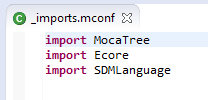
\includegraphics[width=0.4\textwidth]{eclipse_importsFile}
  \caption{\texttt{DictionaryLanguage}'s imports file}
  \label{eclipse:standardImports}
\end{center}
\end{figure}

\texttt{MocaTree} is classified as a standard language, so every eMoflon project includes this specification as a hidden file. Therefore, you're not able to
inspect your target domain directly in Eclipse. Instead, we recommend reviewing Fig.~\ref{ea:mocaTree} which depicts \texttt{MocaTree} in the visual syntax.
Make sure you understand the classes and references before continuing.

\begin{enumerate}

\item[$\blacktriangleright$] Let's establish the TGG we'll use to transform between  \texttt{MocaTree} and\texttt{Dictionary}. Right-click on
\texttt{MyWorkingSet}, and navigate to ``New/ TGG.''

\item[$\blacktriangleright$] Name the package \texttt{DictionaryCodeAdapter}, setting the source as \texttt{MocaTree} and
target as \texttt{DictionaryLanguage} (Fig.~\ref{eclipse:newTGGProject}).

\begin{figure}[htbp]
\begin{center}
  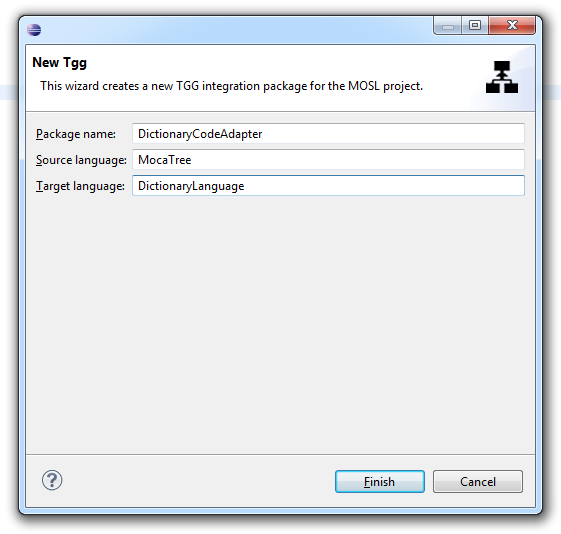
\includegraphics[width=0.9\textwidth]{eclipse_dictionaryCodeAdapterTGGProject}
  \caption{Settings for our TGG}
  \label{eclipse:newTGGProject}
\end{center}
\end{figure}

\item[$\blacktriangleright$] A \texttt{schema.sch} file should have automatically opened in the editor. To ensure this TGG package is successfully generated as
a TGG, let's add something to this by creating our first correspondence type. Specify one between a tree's \texttt{Folder} instance, and a dictionary's
\texttt{Library} as depicted in Fig~\ref{eclipse:firstSchema}.\footnote{For details on this correspondence metamodel and how to build types
between classes, refer to Part IV, Section 3.} Don't forget -- you can use eMoflon's auto-completion feature here!

\begin{figure}[htbp]
\begin{center}
  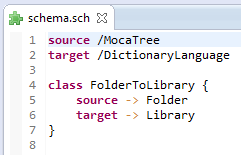
\includegraphics[width=0.5\textwidth]{eclipse_schemaStart}
  \caption{A first correspondence type between domains}
  \label{eclipse:firstSchema}
\end{center}
\end{figure}

\item[$\blacktriangleright$] Save and build your project! Confirm the generated project has a solid black hexagon symbol, not a plug icon
overlaying the folder. This shape indicates the \texttt{Dictionary} is a TGG Package, and is not a standard Ecore project (the default generation type).

\end{enumerate}
